\documentclass{article}

\usepackage{graphicx}
\begin{document}

\title{Presentación del primer proyecto de programación}
\author{Michell Viu Ramirez}
\date{Julio, 2023}
\maketitle

\begin{figure}[h]
    \centering
    
\includegraphics[width=3cm]{matcom.jpg}
\end{figure}

\newpage
\tableofcontents

\newpage
\section{Introducción}
\textbf{¿} Qué es \textit{Moogle!} \textbf{?}\\
Moogle! es una aplicación totalmente original cuyo propósito es buscar 
inteligentemente un texto en un conjunto de documentos.
Es una aplicación web, desarrollada con tecnología .NET Core 6.0, específicamente 
usando Blazor como framework web para la interfaz gráfica, y en el lenguaje C\#.
La idea original del proyecto es buscar en un conjunto de archivos de texto (con extensión `.txt`)

\begin{figure}[h]
    \centering
    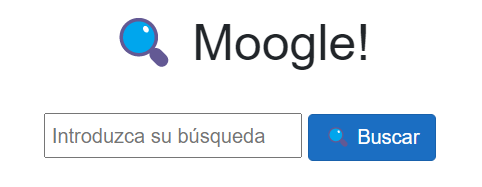
\includegraphics[width=6cm]{Moogle.png}
\end{figure}

\section{Arquitectura del proyecto}
El nuevo proyecto cuenta con tres clases nuevas
\begin{itemize}
    \item Clase \textit{Documentos}: Esta clase consta de seis propiedades y de nueve métodos, la propiedad
     `nombreDocumento` de tipo string que represeta el nombre del "Documento",la propiedad `score` de tipo 
     float que representa la relevancia de ese "Documento" para una búsqueda dada, la propiedad 
     `cantidadDePalabras` de tipo int que representa la cantidad de palabras del "Documento", 
     la propiedad `contenido` de tipo string[ ] que representa cada palabra del "Documento" y 
     la propiedad `snippet` de tipo string que representa una porción del "Documento" para una 
     búsqueda dada y la propiedad `palabrasTF` de tipo Dictionary(string,int) que representa la 
     cantidad de veces que aparece una palabra en un "Documento". En su contructor se recibe como
     parámetros un string `nombreDoc`, un int `longitud` y un string[ ] `contenido`, las propiedades
     nombreDocumento, cantidadDePalabras y contenido reciben en el constructor los valores de nombreDoc,
     longitud y contenido respectivamente,score se inicializa en 0, snippet se inicialeza en "" 
     y palabrasTF en un nuevo Dictionary(string,int). Los métodos de esta clase son get y set que se utilizan
     para obtener o modificar el valor de algunas propiedades.
    \item Clase \textit{Matriz}: Esta clase consta de una propiedad de tipo double[,], nueve métodos que cada uno 
    de ellos realiza una operación entre matrices y/o vectores. En su constructor recibe un matriz de tipo
    double(double[,]).
    \item Clase \textit{MetodosAdicionales}: Es una clase estática que consta de dos métodos:
    \begin{enumerate}
        \item Método \textit{ArrayQuery}: recibe como parémetro un string query y devuelve un array de tipo 
        string, su función en el proyecto es normalizar el string query así como convertirlo en un array de 
        tipo string y eliminar términos que no son relevantes para la búsqueda como preposiciones, conjunciones
         y artículos.
        \item Método \textit{SubString}: recibe como parámetros un array de tipo string, un int "inicio", 
        un int "fin"y un string "término", y retorna un string. Su función es crear el "snippet" del 
        "término" buscado en caso de que aparezca en el documento.
    \end{enumerate}
\end{itemize}

\begin{figure}[h]
    \center
    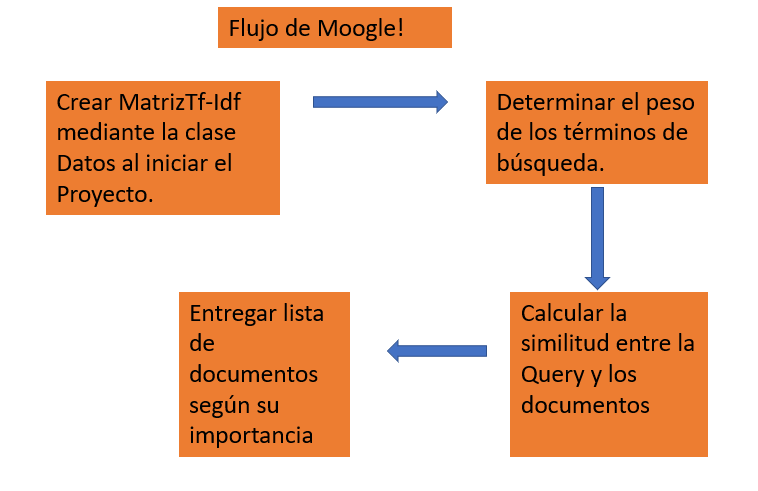
\includegraphics[width=12cm]{flujoM.png}
    \caption{Flujo del proyecto}
\end{figure}

\section{Conclusiones}
\begin{itemize}
    \item Éxito en la implementación del proyecto.
    \item Cumplimiento de los objetivos establecidos.
    \item Aprendizaje de nuevas herramientas y conceptos.
    \item Oportunidades de mejoras y trabajo futuro.
\end{itemize}

\end{document}